\documentclass[aspectratio=169]{beamer}
\usepackage{tikz}
% numbering=none,counter,fraction - frame number at bottom right
\usetheme[block=fill,numbering=none,progressbar=foot]{metropolis}           % Use metropolis theme

\definecolor{RoyalBlue}{cmyk}{1, 0.50, 0, 0}
\definecolor{BgBlue}{cmyk}{1, 0.5, 0,0.8}

\setbeamercolor{progress bar}{fg=RoyalBlue!100, bg=RoyalBlue!30}
\setbeamercolor{frametitle}{bg=BgBlue!100}
\title{AIOLI - AI Open Lab Initiative}
\date{\today}
%\author{Tobias Weis - weis@ccc.cs.uni-frankfurt.de}
\author{\texorpdfstring{\url{[mundt,weis]@ccc.cs.uni-frankfurt.de}}{Tobias Weis}}
\institute{Systems Engineering for Computer Vision}

%%%%%%%%%%%%%%%%%%% TITLE RIGHT
\makeatletter
\setbeamertemplate{title page}{

  \begin{minipage}[b][\paperheight]{\textwidth}

    %\centering
    \raggedleft
    \ifx\inserttitlegraphic\@empty\else\usebeamertemplate*{title graphic}\fi
    \vfill%
    \ifx\inserttitle\@empty\else\usebeamertemplate*{title}\fi
    \ifx\insertsubtitle\@empty\else\usebeamertemplate*{subtitle}\fi
    %\usebeamertemplate*{title separator}
    \ifx\beamer@shortauthor\@empty\else\usebeamertemplate*{author}\fi
    \ifx\insertdate\@empty\else\usebeamertemplate*{date}\fi
    \ifx\insertinstitute\@empty\else\usebeamertemplate*{institute}\fi
    \vfill
    \vspace*{1mm}
  \end{minipage}
}

\setbeamertemplate{title}{
  \raggedleft%
  \linespread{1.0}%
  \inserttitle%
  \par%
  \vspace*{0.5em}
}
\setbeamertemplate{subtitle}{
  \raggedleft%
  \insertsubtitle%
  \par%
  \vspace*{0.5em}
}
\makeatother

%%%%%%%%%%%%%%%%%%%%%%%

\begin{document}


{\usebackgroundtemplate{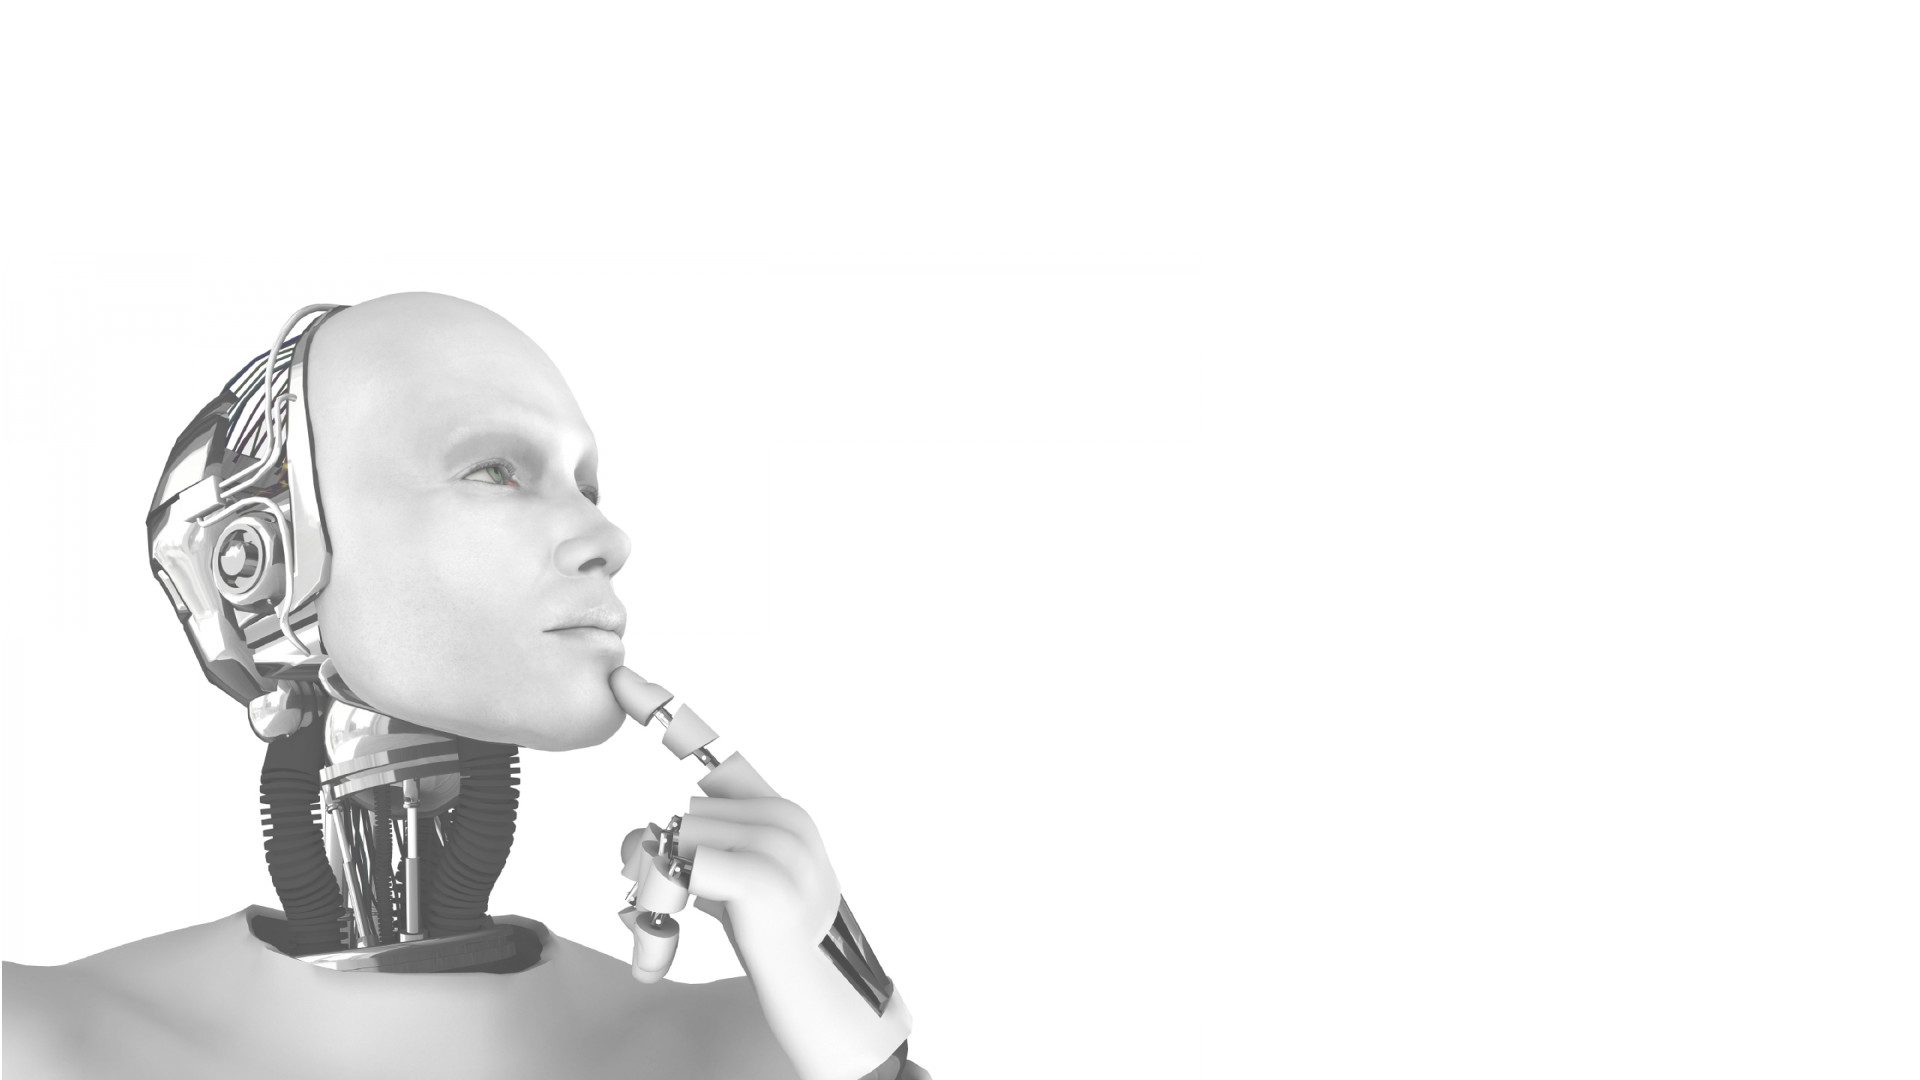
\includegraphics[width=\paperwidth]{images/ai_bg.jpg}}
\maketitle}

%\usebackgroundtemplate{
%}

%%%%%%%%%%%%%%%%%%%%%%%%%%%%%%%%%%%%%%%%%%%%%%%%%%%%%%%%%%%%%%%%%%%%%%%%%%%%%%%%
%                       DEFINITIONS
%%%%%%%%%%%%%%%%%%%%%%%%%%%%%%%%%%%%%%%%%%%%%%%%%%%%%%%%%%%%%%%%%%%%%%%%%%%%%%%%
\section{Agenda}
	\begin{frame}{Agenda}
		\tableofcontents

%	    \begin{itemize}
%		    \item Mission statement
%		    \item Get to know each other
%		    \item What is AI/ML?
%		    \item Presentations/Workshops for next session
%		    \item Open discussion
%	    \end{itemize}
	\end{frame}

\section{Mission statement}
	\begin{frame}{Mission statement}
		We want AIOLI to become a foundation for
		\begin{itemize}
			\item presenting, finding ideas or partners for cool projects,
			\item hosting or attending interesting workshops,
			\item open discussions and
			\item sharing and extending knowledge
		\end{itemize}
		\vfill
		What we \textbf{do not} want it to become:
		\begin{itemize}
			\item No direct connection to curriculum, no CP
			\item No journal club
		\end{itemize}
	\end{frame}

	\begin{frame}{Mission statement - FAQ}
		\begin{block}{Which kind of projects?}
			Whatever you can think of, as long as it is related to ML/AI. This will be a permanent part of the agenda.
		\end{block}

		\begin{block}{What do you mean by workshop?}
			Hands-on sessions by any experienced person willing to present and lead through a project/implementation.
		\end{block}

	\end{frame}

\section{Get to know each other}
	\begin{frame}{Hi, my name is...}
		Tell us a little bit about yourself: 
		\begin{itemize}
			\item your name, 
			\item field of study,
			\item interests/experiences in this domain,
			\item expectations/hopes for the next sessions
		\end{itemize}
	\end{frame}

\section{What is AI/ML}
	\begin{frame}{What is AI/ML?}
		% TODO: put some content here, or start the other presentation
	\end{frame}

\section{Topics for upcoming sessions - Choose wisely}
	\begin{frame}{Topics for upcoming sessions - Choose wisely}
		\begin{itemize}
			\item T: Trafficsigns
			\item T: Kaggle - SanFrancisco crimes
			\item T: RoboCup - Image processing
			\item T: Robot localization + navigation
		\end{itemize}
	\end{frame}

\section{EOP}
\end{document}
